\section{Tutorium 10.04.25}
\label{sec:10_04_25}

\subsection{Organisatorisches}
\begin{itemize}
\item Festlegung des allgemeinen Tutoriumtermins. Ort: Voraussichtlich wieder Geomatikum, wenn Raum verfügbar.
\item Fahrplan MfP4: Differentialgeometrie, Funktionentheorie, Funktionalanalysis
\item Wünsche für das Tutorium? Vergleich letzte Semester, konkrete Vorstellungen, etc.
\item MathNet-Wolke, Moodle, Homepage, Telegram-Gruppe
\end{itemize}

\subsection{Literaturempfehlungen}
Zur Differentialgeometrie kennt ihr bereits meine Empfehlungen von letztem Semester.
Zur Funktionentheorie:
\begin{itemize}
\item Jänich, \href{https://link.springer.com/book/10.1007/3-540-35015-2}{Funktionentheorie}: Sehr angenehm zu lesendes Buch, vor allem, wenn man vielleicht auch an gut geschriebenen Büchern und Anekdoten Spaß hat. 
\item Salamon, \href{https://link.springer.com/book/10.1007/978-3-0348-0169-0}{Funktionentheorie}: Das Buch basiert auf Ahlfors, Complex Analysis, einem beachtlich guten Standardwerk im englischen Raum. Etwas trockener als Jänich, eher im typischen Mathe-Stil.
\item Needham, \href{https://umv.science.upjs.sk/hutnik/NeedhamVCA.pdf}{Visual Complex Analysis}: Das (englischsprachige) Buch kann man am besten nebenher lesen, wenn man sich für die geometrische Intuition hinter der Funktionentheorie interessiert.
\end{itemize}
Zur Funktionalanalysis:
Hier ist das Skript kaum zu schlagen, da die Themenwahl wirklich sehr speziell auf das Notwendigste für die Physik gelegt wurde. Die meisten Mathebücher würden die Konzepte aus dem zweiten Semesterteil auf zwei ganze Semester aufteilen. Und dazu kommt noch mehr Maßtheorie\dots. Nichtsdestotrotz, ein bisschen was fällt mir ein:
\begin{itemize}
\item Kaballo, \href{https://link.springer.com/book/10.1007/978-3-662-54748-9}{Grundkurs Funktionalanalysis}: Das Buch ist aus einem MfP-ähnlichen Modul entstanden und daher einigermaßen geeignet. Allgemein ist das Buch relativ nett geschrieben.
\item Hall, \href{https://link.springer.com/book/10.1007/978-1-4614-7116-5}{Quantum Theory for Mathematicians}: Hier wird die Funktionalanalysis aus Sicht der Physik mit mittelmäßigem mathematischen Anspruch betrachtet. Mathematisch streng veranlagte Leute können mit dem Buch oft nicht so viel anfangen, manchen gereicht es aber auch zur Rettung. Einfach mal reinlesen :)
\end{itemize}
Im Allgemeinen ist MfP4 meiner Erfahrung nach, vor allem wenn noch Differentialgeometrie abgefragt wird, sehr gut machbar, vor allem im Vergleich zu den sehr dichten MfP2- und MfP3-Modulen. Erfahrungsgemäß mögen viele die Funktionentheorie sehr und können damit gut umgehen. Funktionalanalysis fällt hingegen meist schwer, da das Thema vielen weniger intuitiv scheint. Im besten Fall findet man aber an beidem Gefallen, im schlimmsten Fall kommt man mit DiffGeo und Funktionentheorie sicher durch die Klausur.

\subsection{Wiederholung - Komplexe Zahlen}
Mit Sicherheit erinnert ihr euch noch gut an die komplexen Zahlen:
\begin{definition}{Komplexe Zahlen}{komplexezahlen}
Der Körper $(\C, +, \cdot)$ mit
\begin{equation}
\C := \{(a,b) \in \R \mid a,b \in \R\}
\end{equation}
und den Operationen
\begin{equation}
\begin{split}
+: \C \times \C &\to \C\\
(a,b), (c,d) &\mapsto (a,b) + (c,d) := (a+c,b+d),
\end{split}
\end{equation}
genannt Addition, und
\begin{equation}
\begin{split}
\cdot: \C \times \C &\to \C\\
(a,b),(c,d) &\mapsto (a,b) \cdot (c,d) := (ac-bd, ad+bc),
\end{split}
\end{equation}
genannt Multiplikation, nennen wir den Körper der \textbf{komplexen Zahlen}. Die Zahl $a=\Re(a,b)$ heißt \textbf{Realteil}, die Zahl $b=\Im(a,b)$ \textbf{Imaginärteil} von $z$. 
\end{definition}
Meist führt man die \textit{komplexe Einheit} $i$ ein, sodass $(a,b)=a+bi$ für $i^2:=-1$ gilt. Dies erleichtert Rechnungen, ist aber rein symbolischer Natur. Fundamental ist, dass hier ein Körper vorliegt: Sowohl $(\C, +)$ als auch $(\C^\ast, \cdot)$ sind Gruppen (das könnt ihr gerne zur Übung nachprüfen, vor allem die Inversen sollte man einmal konstruiert haben). Bereits aus MfP1 kennt ihr die \textit{komplexe Konjugation}
\begin{equation}
\begin{split}
\overline{\cdot}: \C &\to \C\\
z = a+bi &\mapsto \overline{z} := a-bi.
\end{split}
\end{equation}
Geometrisch entspricht dies einer Spiegelung an der reellen Achse. Auf $\C$ definieren wir außerdem den \textit{Absolutwert} oder \textit{Betrag} durch
\begin{equation}
\begin{split}
|\cdot |: \C &\to \C\\
z &\mapsto |z| := \sqrt{z \overline{z}} = \sqrt{\Re(z)+\Im(z)}
\end{split}
\end{equation}
mit einigen wichtigen Eigenschaften:
\begin{enumerate}[({M}1)]
\item Positivität: $|z| \geq 0$ mit $|z| = 0 \iff z=0$
\item Multiplikativität: $|z_1z_2| = |z_1||z_2|$
\item Subadditivität (Dreiecksungleichung): $|z_1+z_2| \leq |z_1| + |z_2|$.
\end{enumerate}
Sowohl die Multiplikativität als auch die Subadditivität kann man induktiv auf beliebige \red{endliche} Produkte bzw. Summen ausweiten.\\
Damit erhalten wir eine Möglichkeit, aus geometrischen Überlegungen verschiedene Formen für komplexe Zahlen herzuleiten. Ausgehend von der \textit{kartesischen Form} $z=a+bi$ definieren wir den \textbf{Radius} von $z$ als $r := |z|$. Das \textbf{(Haupt-)Argument} von $z$ ist dessen eingeschränkter Polarwinkel $\phi \in (-\pi, \pi]$, das aus trigonometrischen Überlegungen hergeleitet werden kann. Damit erhalten wir die \textit{Polarform} und mit der Eulerschen Formel auch die \textit{trigonometrische Form}:
\begin{equation}
z = r \exp(i\phi) = r(\cos \phi + i \sin \phi).
\end{equation} 
\begin{figure}[H]
\centering
\begin{tikzpicture}[scale=3]
	\draw[step=.5cm, gray, very thin, dotted] (-1.4,-1.4) grid (1.4,1.4);
	\foreach \x/\xtext in {-1, 1}
		\draw (\x,-1pt) -- (\x, 1pt) node[anchor=north] {$\xtext$};
	\foreach \y/\ytext in {-1, 1}
		\draw (-1pt, \y) -- (1pt, \y) node[anchor=east, left=2pt] {$\ytext$};
	\draw[->] (-1.5,0) -- (1.5,0);
	\draw[->] (0,-1.5) -- (0,1.5);
	\draw (0,0) circle [radius=1cm];
	\draw (.5cm,0) arc [start angle=0, end angle=40, radius=.5cm] node[right=1pt,pos=0.5] {$\phi$};
	\draw[red] (40:1cm) -- node[right=1pt, thick] {$\sin \phi = \Im(z)$} (40:1cm |- 0,0);
	\draw[blue] (0,0) -- node[below=4pt,pos=0.5, thick] {$\cos \phi = \Re(z)$} (40:1cm |- 0,0);
	\draw (0,0) -- node[above=2pt, thick] {$r$}  (40:1cm) node[black, right=1pt] {$z$};
	\filldraw[black] (40:1cm) circle [radius=0.5pt];
\end{tikzpicture}
\caption{Die Einheitskreislinie $\S^1 \hookrightarrow \C$ mit der komplexen Zahl $z=r\exp(i\phi)$.}
\end{figure}
Nicht immer ist es ganz so einfach, das Argument aus der kartesischen Form zu ermitteln. Wir illustrieren dies mal wie folgt:
\begin{figure}[H]
\centering
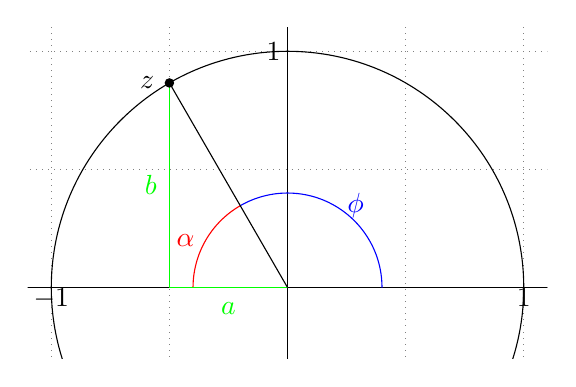
\begin{tikzpicture}[scale=3]
	\clip (-1.1, -0.3) rectangle (1.1, 1.1);
	\draw[step=.5cm, gray, very thin, dotted] (-1.4,-1.4) grid (1.4,1.4);
	\foreach \x/\xtext in {-1, 1}
		\draw (\x,-1pt) -- (\x, 1pt) node[anchor=north] {$\xtext$};
	\foreach \y/\ytext in {-1, 1}
		\draw (-1pt, \y) -- (1pt, \y) node[anchor=east, left=2pt] {$\ytext$};
	\draw[->] (-1.5,0) -- (1.5,0);
	\draw[->] (0,-1.5) -- (0,1.5);
	\draw (0,0) circle [radius=1cm];
	\draw[blue] (.4cm,0) arc [start angle=0, end angle=120, radius=.4cm] node[right=1pt,pos=0.5] {$\phi$};
	\draw[red] (-.4cm,0) arc [start angle=180, end angle=120, radius=.4cm] node[left=.5pt, pos=0.5] {$\alpha$};
	\draw[green] (120:1cm) --  (120:1cm |- 0,0) node[left=1pt,pos=0.5] {$b$} ;
	\draw[green] (0,0) -- node[below=2pt] {$a$} (120:1cm |- 0,0) ;
	\draw (0,0) --   (120:1cm) node[black, left=2pt] {$z$};
	\filldraw[black] (120:1cm) circle [radius=0.5pt];
\end{tikzpicture}
\caption{In diesem Fall lässt sich der Polarwinkel von $z=a+ib$ nicht direkt ableiten. Wir erhalten $\cos \alpha = \frac{|a|}{\sqrt{a^2+b^2}}$ und damit $\phi = \pi - \arccos(\frac{|a|}{\sqrt{a^2+b^2}}) = \arccos(\frac{a}{\sqrt{a^2+b^2}})$. Dabei nutzt man, dass $\arccos(x) = \pi - \arccos(-x)$ gilt.}
\end{figure}
Eine weitere sehr wichtige Ungleichung wollen wir zur Übung beweisen:
\begin{satz}{Cauchy-Schwarz-Ungleichung}{cauchyschwarz}
Seien $x_1, \dots, x_n, y_1, \dots, y_n \in \C$ endlich viele komplexe Zahlen. Dann gilt die \textbf{Cauchy-Schwarz-Ungleichung}
\begin{equation}
\left| \sum_{i=1}^n x_i \overline{y}_i\right|^2 \leq \sum_{i=1}^n |x_i|^2 \sum_{i=1}^n |y_i|^2.
\end{equation}
\end{satz}
\begin{beweis}
Für den Beweis brauchen wir zwei Vorüberlegungen. Erst einmal bemerken wir, dass die Gleichung immer gilt, wenn $\sum_i |x_i|^2 \sum_i|y_i|^2 = 0$, da dann alle $x_i$ oder alle $y_i$ verschwinden müssen. Wir müssen den Beweis also nur noch für $\sum_i |x_i|^2 \sum_i|y_i|^2 > 0$ führen. Die andere Vorüberlegung ist etwas technisch\footnote{Wer denkt, die folgenden Umformungen fielen vom Himmel, kann versuchen, es von vorn nach hinten anzugehen. Dann ist es viel offensichtlicher.} Seien $\alpha, \beta, \gamma, \delta \in \R$. Da Quadrate reeller Zahlen immer positiv sind, stellen wir fest:
\begin{align*}
0 \leq (\alpha \delta- \beta \gamma)^2 &= \alpha^2\delta^2 + \beta^2 \gamma^2 -2\alpha \beta \gamma \delta\\
&= \blue{\alpha^2 \beta^2 - \alpha^2 \beta^2 + \gamma^2 \delta^2 - \gamma^2 \delta^2} +\alpha^2\delta^2 + \beta^2 \gamma^2 -2\alpha \beta \gamma \delta\\
&= (\alpha^2 + \gamma^2)(\beta^2+\delta^2) - (\alpha^2 \beta^2 + \gamma^2 \delta^2 + 2 \alpha \beta \gamma \delta)\\
&= (\alpha^2 + \gamma^2)(\beta^2+\delta^2) - (\alpha \beta + \gamma \delta)^2.
\end{align*}
Umstellen liefert nun eine Ungleichung, derer wir uns später bedienen:
\begin{equation}
(\ast)\, (\alpha \beta + \gamma \delta)^2 \leq (\alpha^2 + \gamma^2)(\beta^2+\delta^2).
\end{equation}
Nun beweisen wir endlich die Ungleichung mit vollständiger Induktion:\\
Für den Induktionsanfang brauchen wir nur (M2):
\begin{equation}
|x\overline{y}|^2 = (|x||\overline{y}|)^2 = |x|^2|y|^2.
\end{equation}
Hier gilt sogar Gleichheit. Die Induktionsvoraussetzung (IV) ist, dass die Aussage für $n-1$ gezeigt ist. Da beide Seiten positiv sind, können wir in der IV die Wurzel ziehen:
\begin{equation}
\left| \sum_{i=1}^{n-1} x_i \overline{y}_i\right| \leq \sqrt{\sum_{i=1}^{n-1} |x_i|^2} \sqrt{\sum_{i=1}^{n-1} |y_i|^2}.
\end{equation}
Für den Induktionsschritt müssen wir die Aussage für $n$ beweisen. Das geht nun relativ schnell:
\begin{align*}
\left| \sum_{i=1}^n x_i \overline{y}_i\right| &= \left| x_n \overline{y}_n + \sum_{i=1}^{n-1} x_i \overline{y}_i\right|\leq |x_n \overline{y}_n| + \left| \sum_{i=1}^{n-1} x_i \overline{y}_i\right|\\
&\leq^\text{\red{IV}} |x_n| |y_n| + \sqrt{\sum_{i=1}^{n-1} |x_i|^2} \sqrt{\sum_{i=1}^{n-1} |y_i|^2} \leq^{\red{(\ast)}} \sqrt{\sum_{i=1}^{n} |x_i|^2} \sqrt{\sum_{i=1}^{n} |y_i|^2}
\end{align*}
Im ersten Schritt haben wir die Dreiecksungleichung ausgenutzt, gefolgt von der Induktionsvoraussetzung. Den letzten Schritt können wir mit unserer Ungleichung $(\ast)$ direkt folgern, indem wir $\alpha:=|x_n|$, $\beta:= |y_n|$, $\gamma:= \sqrt{\sum_{i=1}^{n-1} |x_i|^2}$ und $\delta :=\sqrt{\sum_{i=1}^{n-1} |y_i|^2}$ setzen.
\end{beweis}
\subsection{Funktionentheorie ist \textit{nicht} reelle Analysis in zwei Variablen}
Wenn wir nun zur Analysis auf $\C$ übergehen, ist man leicht verleitet, den $\R-$\red{Vektorraum}-Isomorphismus $\C \cong \R^2$ so zu interpretieren, dass Funktionentheorie doch eigentlich nichts anderes sei als Analysis im $\R^2$. Das ist aber ein fataler Fehler! Der Schlüssel liegt darin, dass auf $\C$ eine andere Struktur, die Multiplikation mit komplexen Zahlen, definiert ist, die über die Vektorraumstruktur des $\R^2$ hinausgeht.\\
In der reellen Analysis war die Erkenntnis, dass sich differenzierbare Funktionen durch ihr Differential annähern lassen, fundamental. Ist $f: \R^2 \to \R^2$ eine beliebige, reell-differenzierbare Funktion, so ist ihr Differential am Punkt $p \in  \R^2$ eine reell-lineare Abbildung
\begin{equation}
\begin{split}
df_p: \R^2 \to \R^2\\
x \mapsto df_p (x).
\end{split}
\end{equation} 
Mit der Wahl einer Basis des $\R^2$ lässt sich das Differential als Matrix
\begin{equation}
Df_p := \left. \mat{\frac{\partial f_1}{\partial x_1}, \frac{\partial f_1}{\partial x_2}}{\frac{\partial f_2}{\partial x_1}, \frac{\partial f_2}{\partial x_2}}\right|_p 
\end{equation}
darstellen, genannt \textit{Funktionalmatrix}. Dies ist also einfach eine Matrix der Form $\mat{\alpha, \beta}{\gamma,\delta}$ mit vier reellen Einträgen.\\
Wie sieht das im Komplexen aus? Ist ein komplex-lineares Differential auch einfach eine beliebige $2 \times 2$-Matrix mit reellen Einträgen? Fangen wir mal mit der komplexen Linearität an:
\begin{definition}{Komplex-Lineare Abbildung}{komplexlinear}
Eine Abbildung $A: \C \to \C$ heißt \textbf{komplex-linear}, falls für alle $z_1,z_2,\lambda, \mu \in \C$ gilt:
\begin{equation}
A(\lambda z_1+\mu z_2) = \lambda A(z_1)+ \mu A(z_2).
\end{equation}
\end{definition} 
Wir fordern für eine Funktion $f: \C \to C$ nun, dass das Differential $df_p: \C \to \C$ nicht bloß linear, sondern komplex-linear ist. Bereits erwähnt habe ich, dass Addition nichts Neues ist. Diese funktioniert auf $\R^2$ und $\C$ völlig analog, nämlich komponentenweise. Neu ist hingegen die Multiplikation mit einer komplexen Zahl, aber was bedeutet das für die darstellende Matrix für das Differential? Wenn wir nur Multiplikation mit komplexen Zahlen betrachten wollen und uns nicht für Addition interessieren, liegt es nahe, erst einmal nur $\C$ mit Multiplikation zu betrachten. Wir gehen es noch langsamer an und schauen, was passiert, wenn wir nur komplexe Zahlen mit Radius $r=1$ zulassen, also die Einheitskreislinie $\S^1 \sub \C$ anschauen. Praktischerweise ist $(\S^1, \cdot)$ eine Gruppe, die einer uns bekannten Gruppe sehr ähnlich sieht. Sind $z_1 = \exp(i\phi_1)$ und $z_2 = \exp(i \phi_2)$ zwei komplexe, normierte Zahlen, so ist ihr Produkt gegeben durch
\begin{equation}
z_1z_2 = \exp(i(\phi_1+\phi_2)).
\end{equation}
Dass sich die Winkel addieren, ist der entscheidende Hinweis für den gesuchten Isomorphismus:
\begin{satz}{Multiplikation ist Rotation}{komplexmat}
Es existiert ein Gruppen-Isomorphismus $(\S^1, \cdot) \cong \so{2}$ zwischen dem Einheitskreis
\begin{equation}
\S^1 := \{x+iy \in \C \mid x^2+y^2=1\} \sub \C
\end{equation}
mit komplexer Multiplikation und der speziellen orthogonalen Matrizengruppe.
\end{satz}
\begin{beweis}
Aus MfP2 wissen wir, dass sich $\so{2}$-Matrizen parametrisieren lassen als
\begin{equation}
\mat{\cos \phi, -\sin \phi}{\sin \phi, \cos \phi} =: R(\phi)
\end{equation}
mit $\phi \in (-\pi, \pi]$. Darauf aufbauend ist der Isomorphismus mit der Polarform schnell konstruiert: Wir behaupten, dass 
\begin{equation}
\begin{split}
\psi: (\S^1, \cdot) &\to \so{2}\\
\exp(i\phi) &\mapsto \mat{\cos \phi, -\sin \phi}{\sin \phi, \cos \phi}
\end{split}
\end{equation}
passt. Dabei haben wir den Einheitskreis in der komplexen Ebene mit komplexen Zahlen des Radius $r=1$ identifiziert. Also fehlen nur noch die Eigenschaften:
\begin{enumerate}[({I}1)]
\item Gruppenhomomorphismus: Seien $\exp(i\phi_1), \exp(i \phi_2) \in \S^1$. Dann gilt:
\begin{align*}
\psi \left( \exp(i\phi_1)\right) \cdot \psi \left(\exp(i \phi_2)\right) &=  \mat{\cos \phi_1 , -\sin \phi_1}{\sin \phi_1, \cos \phi_1}\mat{\cos \phi_2, -\sin \phi_2}{\sin \phi_2, \cos \phi_2}\\
&= \mat{\cos \phi_1 \cos \phi_2 - \sin \phi_1 \sin \phi_2 , -(\sin \phi_2 \cos \phi_1 + \sin \phi_1 \cos \phi_2)}{\sin \phi_1 \cos \phi_2 + \sin \phi_2 \cos \phi_1, -\sin \phi_1 \sin \phi_2 + \cos \phi_1 \cos \phi_2}\\
&= \mat{\cos(\phi_1+\phi_2) , -\sin(\phi_1+\phi_2)}{\sin(\phi_1 + \phi_2), \cos(\phi_1+\phi_2)}=\psi \left( \exp(i\phi_1+\phi_2)\right)\\
&=\psi(\exp(i\phi_1)\exp(i\phi_2)).
\end{align*}
Benutzt haben wir dabei lediglich die beiden gängigen Additionstheoreme.
\item Bijektiv: Das ist tatsächlich trivial, man kann die Inverse von $\psi$ Dank der Parametrisierung von $\so{2}$ direkt ablesen.
\end{enumerate}
\end{beweis}
Das ist doch mal ein Ergebnis. Jetzt wissen wir, dass Multiplikation mit komplexen Einheiten äquivalent zu Rotationen in der Ebene sind. Aber was passiert, wenn man beliebige komplexe Zahlen und nicht nur normierte zulässt? Das Verhalten kennen wir schon aus der linearen Algebra: Multiplikation mit einem reellen Skalar bewirkt eine Streckung oder Stauchung.\\
Komplex-lineare Abbildungen werden also von Matrizen der Form
\begin{equation}
\mat{\alpha, -\beta}{\beta, \alpha}
\end{equation}
repräsentiert. Dies ist eine starke Einschränkung gegenüber dem reellen Fall! Eine komplex-differenzierbare Funktion muss also nicht bloß lokal wie eine reell-lineare Abbildung, sondern sogar wie eine Drehskalierung aussehen. Diese reichere Struktur wird viele, sehr schöne Phänomene in der Funktionentheorie zur Folge haben.\\
Da wir nun so weit sind, bietet sich noch ein Vergleich der Funktionalmatrix mit der neuen Differentialmatrix an: Fassen wir $f: \C \to \C$ auf als $f: \R^2 \to \R^2$ mit $f(x,y) = f_1(x,y)+if_2(x,y)$ und vergleichen, so erhalten wir
\begin{align*}
\alpha &= \frac{\partial f_1}{\partial x} = \frac{\partial f_2}{\partial y}\\
\beta  &= \frac{\partial f_2}{\partial x} = -\frac{\partial f_1}{\partial y}.
\end{align*}
Überraschung (oder auch nicht), das sind die \textbf{Cauchy-Riemannschen Differentialgleichungen}. Diese entsprechen also der Anforderung, dass unsere Funktion komplex-differenzierbar ist.